\providecommand{\topdir}{..}
\documentclass[../main.tex]{subfiles}

\ifSubfilesClassLoaded{
  \externaldocument[main-]{../main}
  \setcounterref{chapter}{main-chap:evaluation}
  \addtocounter{chapter}{-1}
}{}

\externaldocument{\subfix{../00_front_matter/front_matter}}
\externaldocument{\subfix{../01_introduction/introduction}}
\externaldocument{\subfix{../02_lorenz96/lorenz96}}
\externaldocument{\subfix{../03_rayleigh_benard/rayleigh_benard}}
\externaldocument{\subfix{../04_tendencies/tendencies}}
\externaldocument{\subfix{../06_conclusion/conclusion}}
\externaldocument{\subfix{../07_appendix/appendix}}

\begin{document}

\ifSubfilesClassLoaded{
    \frontmatter
    \tableofcontents
    \mainmatter
}{}

\chapter{Online assessment of the parametrised model} \label{chap:evaluation}
\setlength{\epigraphwidth}{0.5\linewidth}
\epigraphhead[0.1\textheight]{
    \epigraph{
        All models are wrong but some are useful.
    }{
        \emph{Robustness in the Strategy of Scientific Model Building} \\
        George Box, 1979
    }
}

In \cref{chap:tendencies}, I analysed the subgrid tendencies and
constructed a statistical model \cref{eqn:scheme_poly} to estimate
them from the coarse model tendencies. In this chapter, I will assess
the performance of the parametrised model obtained by coupling the
statistical model into the coarse \rb{} model.

First, a ``truth'' solution was obtained by running the fine (i.e., $2048
\times 256$; see \cref{tab:final_resolutions}) model for 300 time units,
saving the output at intervals of 0.2 time units. The last snapshot from the
fine model simulation described in \cref{sec:calculation}
(\cref{itm:fine_model}) was used as the initial condition, thus keeping
the data used to test the parametrisation separate from the data used to fit
it. Every snapshot in the truth dataset was then coarse-grained using the
method described in \cref{sec:coarse_graining}; the aim is for the
parametrised model to approximate this coarse-grained truth solution as closely
as possible.

A control solution was obtained by running the unmodified coarse (i.e., $256
\times 64$) model, using the first coarse-grained snapshot of the truth
solution as an initial condition. Output was saved at approximately the
same interval of 0.2 time units.

The equations governing the parametrised model, given schematically by
\cref{eqn:res_tend_parametrised_model}, can be written out explicitly as
\begin{align*}
    \pdiff{\vec{u}}{t} &=
        \begin{pmatrix}
            1 + {\color{red} f_u(z)} & 0 \\
            0 & 1 + {\color{red} f_w(z)}
        \end{pmatrix}
        \left[
            -\vec{u} \cdot \grad \vec{u}
            -\grad \pi
            + \left( \frac{\prandtl}{\rayleigh}\right)^{1/2}
            \left(
                \nabla^2 \vec{u}
                + \tilde{\nu} f(z) |\nabla^2 \vec{u}| \nabla^2 \vec{u}
            \right)
            + \theta \uvec{z}
        \right], \\
    \pdiff{\theta}{t} &=
        (1 + {\color{red} f_\theta(z)}) \left[
            -\vec{u} \cdot \grad \theta
            + (\rayleigh\,\prandtl)^{-1/2}
            \left(
                \nabla^2 \theta
                + \tilde{\kappa} f(z) |\nabla^2 \theta| \nabla^2 \theta
            \right)
        \right], \quad \text{and} \\
    \grad \cdot \vec{u} &= 0,
\end{align*}
where the terms in red distinguish these modified equations from the originals
\crefrange{eqn:hyper_momentum}{eqn:hyper_incompressible}. The
parametrised model was run with the same resolution, time step, initial
condition and output interval as the control.

Unfortunately, when the parametrised model was run with the $f_\theta$,
$f_u$ and $f_w$ that were fitted in \cref{sec:subgrid_modelling}, it
became unstable and crashed within 10 time units. Given the low coefficients
of determination for the $u$ and $w$ fits (\cref{tab:r_squared}), I
chose to set $f_u(z) = f_w(z) \equiv 0$---that is, to only parametrise the
$\theta$ tendency and leave the momentum equation unmodified. This stabilised
the model.

\newpage
\section{Short-term forecast accuracy}
\label{sec:forecast}
I first assess short-term accuracy using the root-mean-square error (RMSE)
of $u$, $w$ and $\theta$, defined by
\[
    \mathrm{RMSE}_\chi(t) = \sqrt{\left\langle
        [\chi_\mathrm{fc}(t) - \chi_\mathrm{truth}(t)]^2
    \right\rangle _{x,z}},
\]
where $\chi = u, w, \theta$, $\chi_\mathrm{fc}$ is the forecast generated by
either the control or parametrised model and $\chi_\mathrm{truth}$ is the
\emph{coarse-grained} truth solution. \cref{fig:rmse} (a-c) compares the RMSE
of the control and parametrised solutions for the first 70 time units of
simulation.

Panel (a) shows that the $\theta$ RMSE of the parametrised model
initially grows at less than half the rate seen in the control, remaining
smaller than the control value for almost 10 time units before surpassing it.
While both models reach a peak RMSE before settling to a steady equilibrium,
the parametrised model takes approximately four times longer to do so. It seems
likely that by reducing the magnitude of $\partial\theta/\partial t$ near the
top and bottom of the domain, the parametrisation preserves the properties of
the thermal boundary layers. These are relatively thick and slowly-evolving in
the coarse-grained truth solution, but are thinned too quickly by the control
model.

For $u$ and $w$, the RMSE of the parametrised model initially increases
at a rate much closer to that of the control model. However, by plotting
the difference between the two and zooming the time axis (panels d-f),
it can be seen that the parametrised model does indeed have a slightly smaller
error.

\begin{figure}[ht]
    \centering
    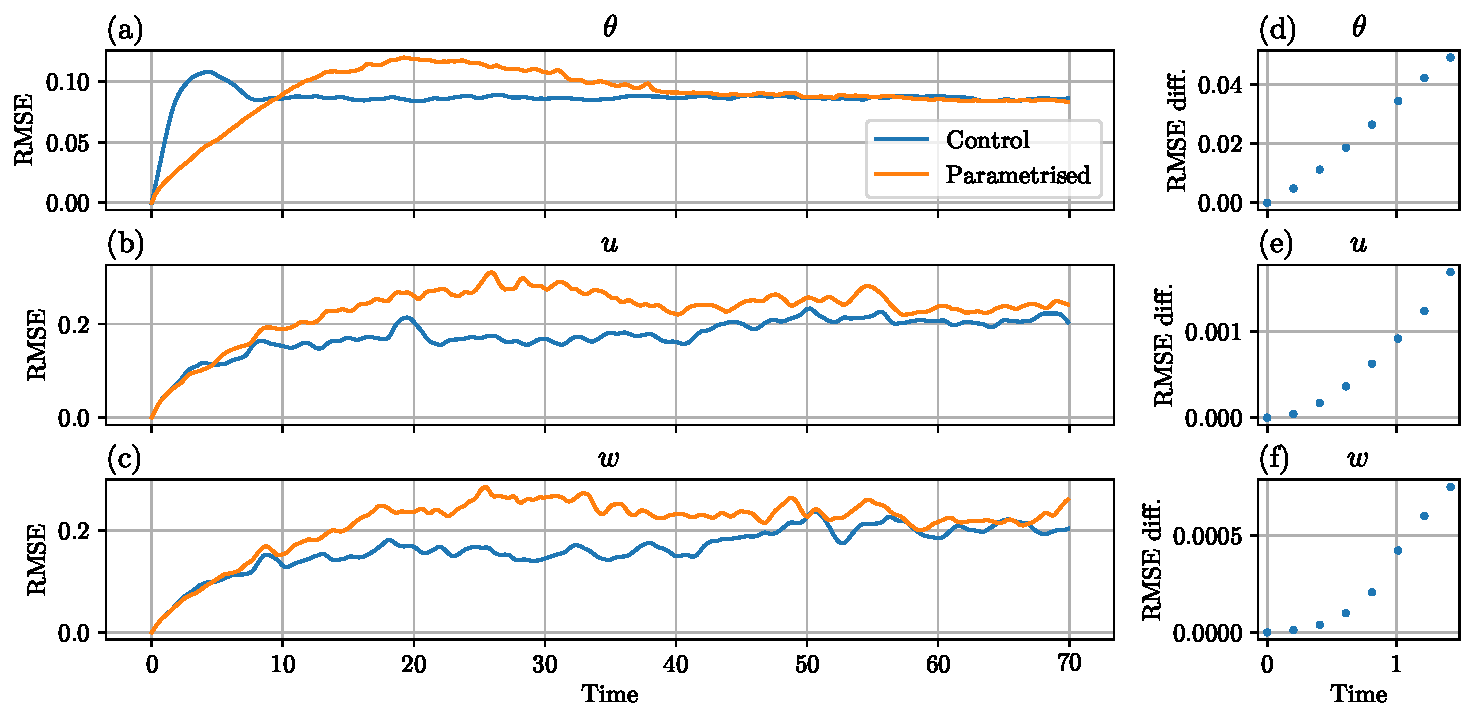
\includegraphics[width=\linewidth]{figures/rmse.pdf}
    \caption{
        \textbf{(a-c):} Root-mean-square error of the control (blue) and
        parametrised (orange) solutions for $\theta$, $u$ and $w$ over
        the first 70 time units of simulation. \textbf{(d-f):} The control
        RMSE minus the parametrised RMSE over the first 1.5 time units,
        confirming that the parametrised solution has lower RMSE in the short
        term.
    }
    \label{fig:rmse}
\end{figure}

Another way to assess short-term accuracy is to calculate domain-averaged
quantities for the parametrised, control and truth solutions and compare them
over time. As in \cref{sec:choose_resolution}, I consider the Nusselt number
$\nusselt$, thermal boundary layer thickness $\delta_\theta$, RMS speed
$u_\mathrm{rms}$, kinetic energy dissipation rate $\epsilon_k$ and thermal
dissipation rate $\epsilon_\theta$, plotting their time series in
\cref{fig:short_term_metrics}. Both the control and parametrised models make
grossly inaccurate predictions for $\delta_\theta$ and $\epsilon_\theta$, but
the parametrised model's predictions are nonetheless closer to the truth for
the first $\sim 20$ time units. Since these are purely thermal quantities,
their improved prediction can be attributed to the nature of the
parametrisation scheme in the same way as the $\theta$ RMSE. The parametrised
model also makes more accurate initial predictions for the other three
quantities, but only for the first $\sim 5$ time units.

\begin{figure}[ht]
    \centering
    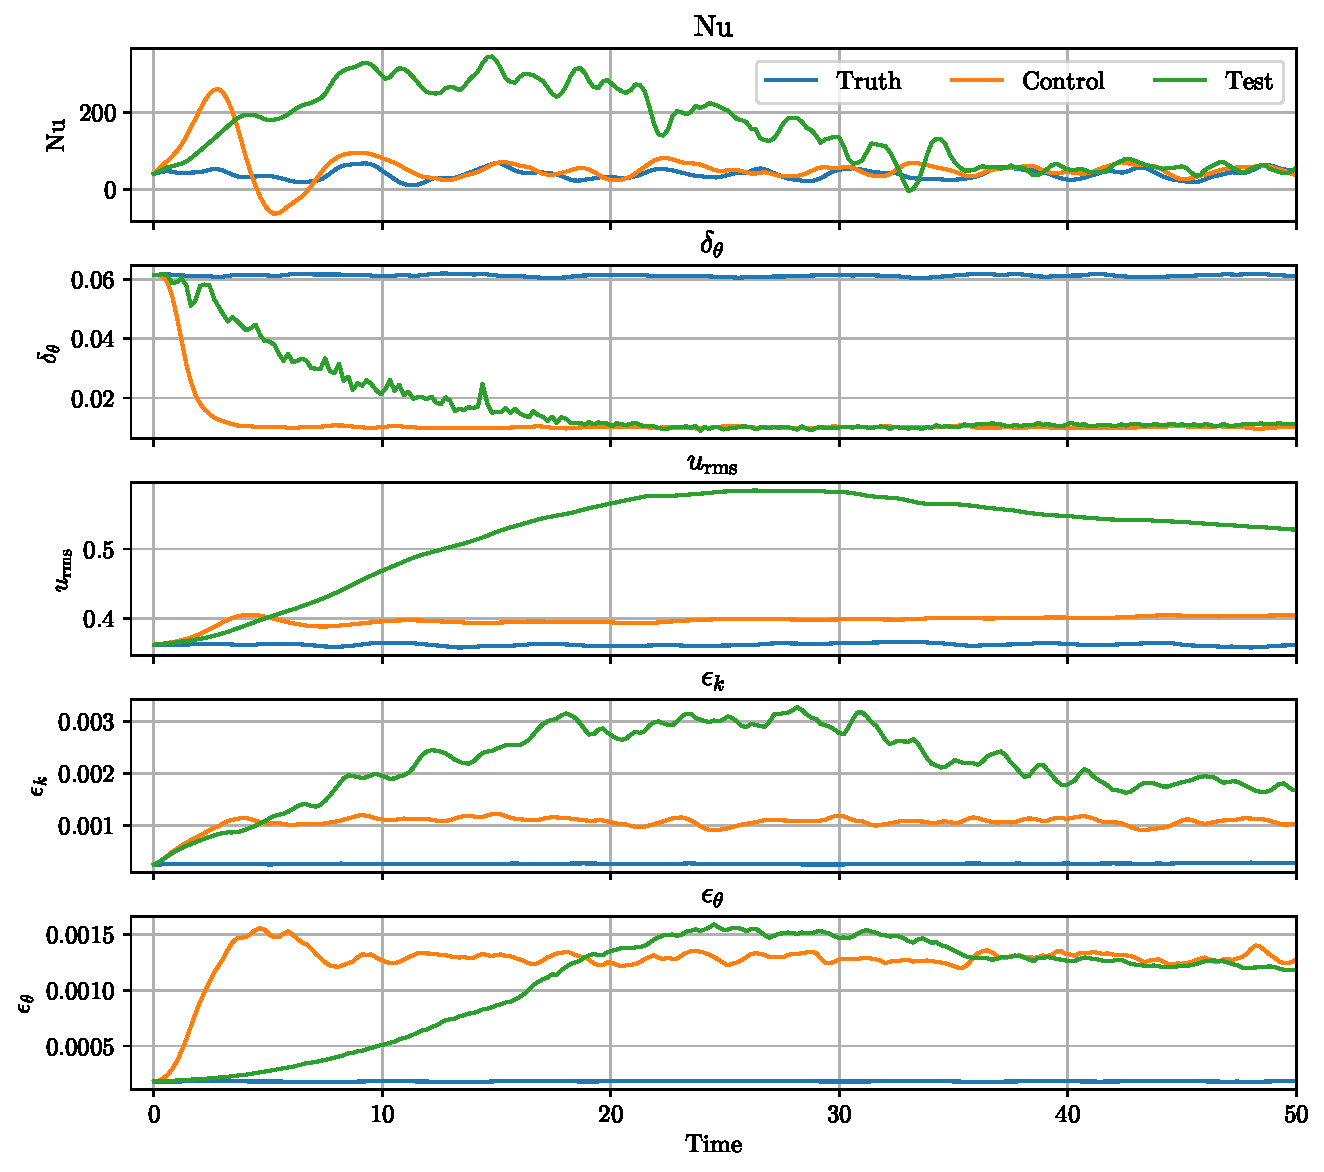
\includegraphics[width=\linewidth]{figures/short_term_metrics.pdf}
    \caption{
        Time series of the Nusselt number $\nusselt$, thermal boundary layer
        thickness $\delta_\theta$, RMS speed $u_\mathrm{rms}$, kinetic energy
        dissipation rate $\epsilon_k$ and thermal dissipation rate
        $\epsilon_\theta$ for the coarse-grained truth (blue), control (orange)
        and parametrised (green) solutions over the first 50 time units.
    }
    \label{fig:short_term_metrics}
\end{figure}

So far, I have shown that the parametrised model is capable of producing
more accurate short-term forecasts than the control if the lead time is
sufficiently short (on the order of a few time units)---a promising result.


\section{Long-term statistical accuracy}
\label{sec:climate}
I next consider the long-term mean properties of the parametrised model once it
is allowed to reach a statistically steady state. This required 1100 time units
of simulation, with the first 800 time units of data being discarded (see
\cref{sec:parametrised_spinup}). For consistency, the control solution was
also extended to 1100 time units. The fine model did not require further
spin-up, having been initialised in a statistically steady state.

It is insightful to first compare the steady-state solutions qualitatively.
\cref{fig:steady_state_vis} shows that the coarse-grained temperature field of
the fine truth solution (panel (a)) is smooth and well-resolved. In particular,
it has a thermal boundary layer thickness on the order of 0.1. The control
model, despite being initialised from a coarse-grained state like the one in
\cref{fig:steady_state_vis}a, reverts to a state where the temperature field is
poorly resolved and the thermal boundary layers are much thinner. Notably, the
parametrised solution is much closer in appearance to the control than the
coarse-grained truth, which it is supposed to represent.

\begin{figure}[ht]
    \centering
    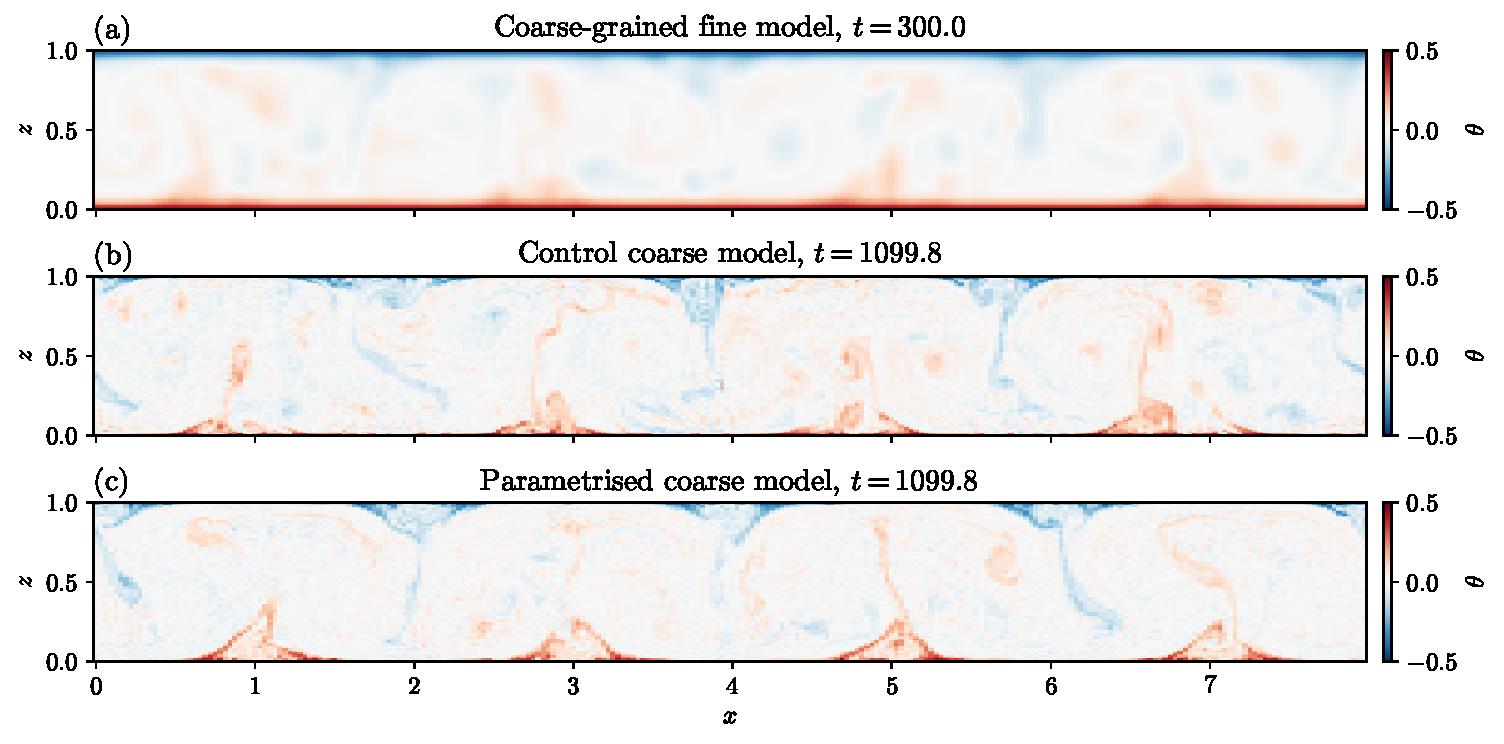
\includegraphics[width=\linewidth]{figures/steady_state_vis.pdf}
    \caption{
        Example temperature snapshots in the statistically steady regime for
        \textbf{(a)} the coarse-grained truth solution (which the parametrised
        solution should ideally resemble), \textbf{(b)} the control solution
        and \textbf{(c)} the parametrised solution.
    }
    \label{fig:steady_state_vis}
\end{figure}

The core issue is the smoothing involved in the coarse-graining operation. On
the one hand, I explained in \cref{sec:coarse_graining} that insufficient
smoothing causes artefacts that mask the subgrid tendency signal, making it
more difficult to model the subgrid tendencies. On the other hand,
\cref{fig:steady_state_vis} shows that the natural state of the coarse model is
not smooth. By parametrising the $\theta$ subgrid tendency, I have attempted to
force the coarse model towards the coarse-grained truth solution, and although
this is successful for a short time (as shown in \cref{sec:forecast}), the
parametrised model eventually settles to a state that is grossly
unrepresentative of the target. It is clear that future work will need to
consider more sophisticated parametrisation schemes in order to resolve this
problem. Such a scheme might contain a diffusion term to further smooth
the coarse solution.

Despite the above issues, I proceed to perform a similar analysis to
\cref{sec:choose_resolution}, calculating the time averages of $\nusselt$,
$\delta_\theta$, $u_\mathrm{rms}$, $\epsilon_k$ and $\epsilon_\theta$ over 300
time units for the coarse-grained truth, control and parametrised solutions. I
stress that the high-resolution truth solution was first coarse-grained before
the metrics were calculated. Uncertainties were estimated using the same method
of running means \cref{eqn:running_mean} and rolling means
\cref{eqn:rolling_mean} with a 150-time-unit window.

\cref{fig:stats} shows that parametrisation has resulted in a statistically
significant improvement across all five metrics, approximately halving the
relative error for $\nusselt$ and $u_\mathrm{rms}$. Both the control and
parametrised solutions have very large errors for $\delta_\theta$ ($\sim -80
\%$), $\epsilon_k$ ($\sim 300 \%$) and $\epsilon_\theta$ ($\sim 500 \%$)---an
unsurprising result, given the issue discussed earlier in this section---but
the relative errors of the parametrised solution are nonetheless smaller than
those of the control.

\begin{figure}[ht]
    \centering
    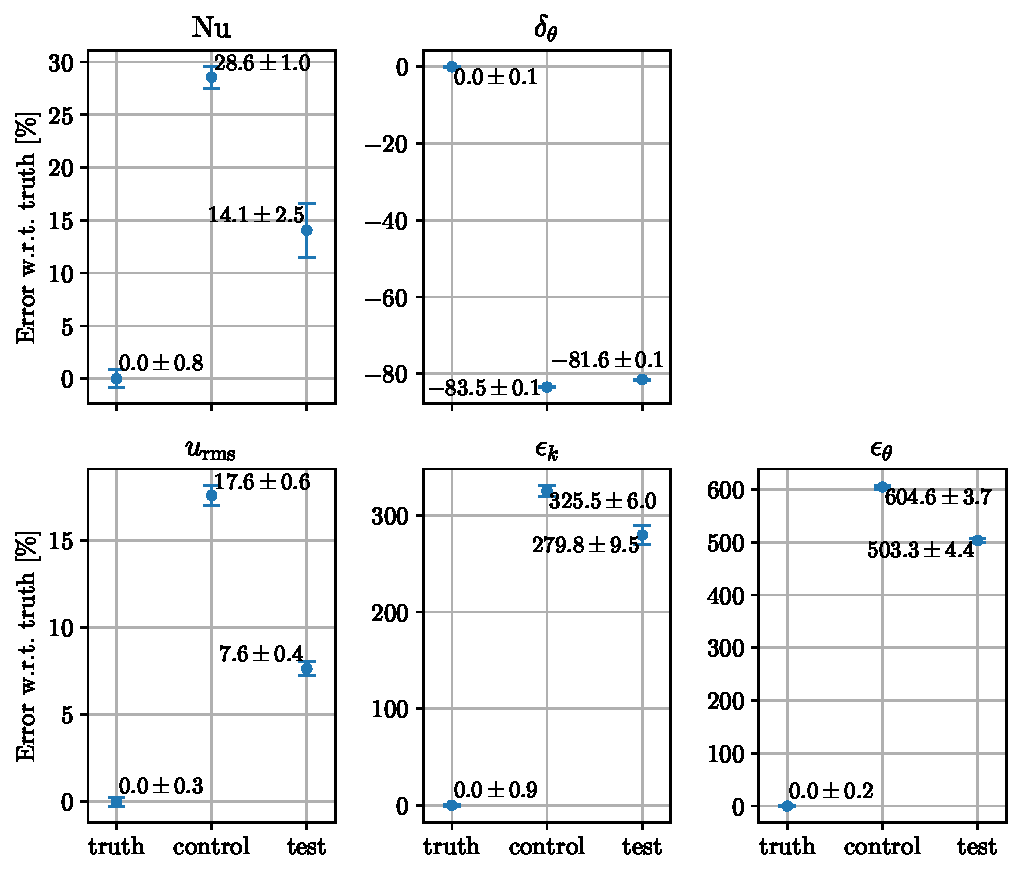
\includegraphics[width=0.7\linewidth]{figures/stats.pdf}
    \caption{
        Time-averaged Nusselt number $\nusselt$, thermal boundary layer
        thickness $\delta_\theta$, RMS speed $u_\mathrm{rms}$, kinetic energy
        dissipation rate $\epsilon_k$ and thermal dissipation rate
        $\epsilon_\theta$ for the coarse-grained truth, control and
        parametrised (``test'') solutions. Values are expressed as percentage
        errors relative to truth.
    }
    \label{fig:stats}
\end{figure}

Given that the parametrised solution is generally unrepresentative of the
coarse-grained truth, one may alternatively ask how close its long-term
statistics are to those of the \emph{uncoarsened} high-resolution truth data. I
repeat the previous analysis, now calculating the truth solution metrics
without first coarse-graining the data. \cref{fig:stats_vs_fine} shows that
parametrisation produces a statistically significant reduction in the magnitude
of the relative error for $\nusselt$, $\delta_\theta$ and $u_\mathrm{rms}$.
There is no significant change in magnitude (but a change of sign) for
$\epsilon_k$ and an increase in magnitude with change in sign for
$\epsilon_\theta$. This is a surprising result because the parametrisation
scheme is not explicitly designed to improve the coarse model in comparison to
the uncoarsened fine model (only the coarse-grained fine model). In fact, this
type of improvement is arguably more useful for practical applications; to give
an analogy, a coarse-resolution climate model that directly reproduces the
spatially-averaged statistics (surface temperature, precipitation rate, etc.)
of a finer model could be more useful than one that reproduces those of the
coarsened and smoothed fine model output.

\todo{summary?}

\begin{figure}[ht]
    \centering
    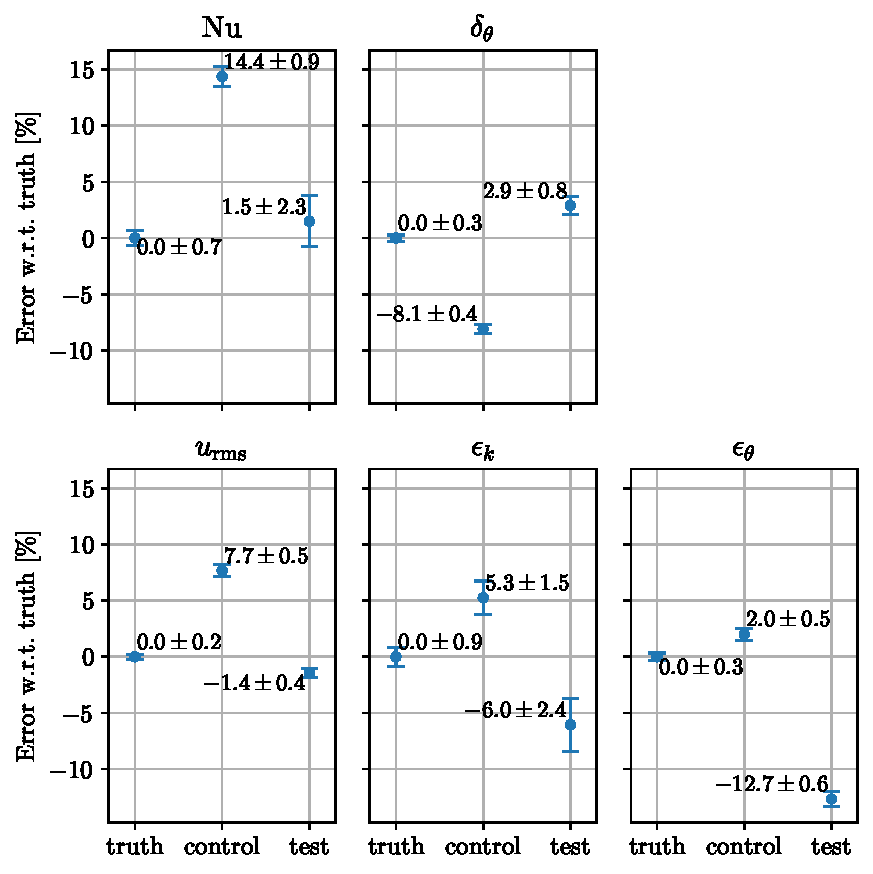
\includegraphics[width=0.6\linewidth]{figures/stats_vs_fine.pdf}
    \caption{
        As for \cref{fig:stats}, except that the truth values are computed
        \emph{without} first coarse-graining the high-resolution data.
    }
    \label{fig:stats_vs_fine}
\end{figure}

\ifSubfilesClassLoaded{%
    \emergencystretch=5em
    \printbibliography{}
}{}

\end{document}
